\section{Teknologibeskrivelse}
%\begin{itemize}
%	\item Hvad består teknologien af?
%	\begin{itemize}
%		\item Hvilke dele består den af? (Hardware og software)

Overordnet består et Fitbit Flex aktivitetsarmbånd af en flex tracker, oplader kabel, trådløs synkroniserings dongle og armbånd til flex tracker \citep{fitbitflex}. Disse kan ligeledes ses af \autoref{fig:fitbitflexindhold}. 
\end{enumerate}

\begin{figure}[H]
	\centering
	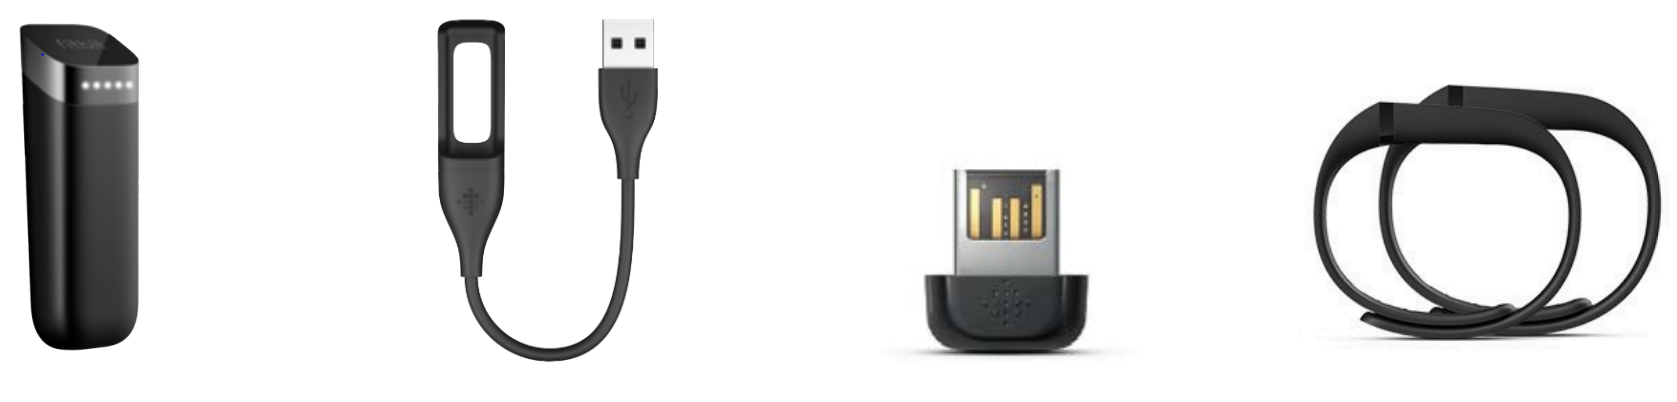
\includegraphics[width=0.6\textwidth]{figures/fitbitflexindhold}
	\caption{Fra venstre mod højre ses flex tracker, oplader kabel, trådløs synkroniserings dongle, armbånd \citep{fitbitflex}.}
	\label{fig:fitbitflexindhold}
\end{figure}

Fitbit Flex er i stand til at måle antal skridt, forbrændte kalorier, afstand dækket, minutter brugeren er aktiv og længden samt kvalitet af søvn. 
For at brugeren kan se den registrerede aktivitet som er blevet opsamlet af armbåndet, skal dette synkroniseres med en kompatibel enhed, da armbåndet kun besidder et display bestående af fem LED'er. %(HVAD BETYDER DET SÅ?? HVIS DER ER 5 STYREDE LED'ER HVAD VISES SÅ??)  
Denne synkronisering foregår trådløst, ved brug af bluetooth low energy og kan forgå mellem forskellige enheder som for eksempel smartphone og computer. 
Synkronisering mellem flex tracker og computer kræver dog anvendelse af den trådløs synkroniserings dongle, der ses af \autoref{fig:fitbitflexindhold}.
Forudsætninger for, at data kan synkroniseres er, at en kompatibel enhed har den korrekte applikation installeret, hvor synkroniseringen ellers sker automatisk idet applikationen åbnes.  
Yderligere skal der oprettes en brugerkonto på www.fitbit.com, hvor brugeren oplyser personlig info: køn, alder, højde og vægt. Dette er nødvendigt i forhold til optimering af dataopsamling og estimering af forbrændte kalorier.  
Gennem applikationen visualiseres den registrerede aktivitet, hvor brugeren har mulighed for at se data fra starttidspunktet for anvendelsen af armbåndet. Data kan også observeres via  Fitbits hjemmeside, hvor det er muligt at logge ind via brugerkontoen. 
Til den daglige aktivitet har brugeren mulighed for at sætte bestemte mål, hvortil det angives, hvor langt brugeren er fra at nå det givne fysiske mål, ved hjælp af de fem LED'er på armbåndet, i løbet af dagen. Denne funktion aktiveres når brugere trykker 2 gange på armbåndet. % (HVOR MANGE GANGE PÅMINEDS PATIENTEN DETTE??).
Fitbit Flex armbåndet er ikke i stand til at visualisere batteriniveauet for armbåndet, dette kan dog ses ved brug af applikationen. 
Hukommelsen i flex trackeren tillader detaljeret data at blive lagret i perioder op til 7 dage og består af minut til minut målinger.  
Yderligere lagres summeringer af daglig aktivitet i op til 30 dage. 
%(VIL DET SIGE AT HVIS MAN IKKE SYNKRONISERER, SÅ LAGRES DATA PÅ ENHEDEN, OG EFTER 7 DAGE SLETTES DEN FØRSTE AF DE 7 DAGE (GEMMES MÅSKE SOM EN SUMMERING AF DAGEN FOR DE 30 DAGE) ELLER HVORDAN FUNGERER DET? : jaa hvordan man.)) 
Ved jævnlig synkronisering er det muligt for brugeren at bevare detaljeret data, da informationen tilknyttes brugerkontoen. 
Fitbit anbefaler én daglig synkronisering, dog er det ikke en nødvendighed \citep{fitbitflex}. 

Armbåndet er vandafvisende (ned til 10 meter) 

\textbf{SLEEP MODE}

% Hvordan udregnes de reelle trackingsværdier, kalorier, afstand mm. 

\subsection{Hardware (for flex trackeren)}
(MÅSKE STARTE AFSNITTET MED DEN HER BESKRIVELSE AF HARDWAREN? SÅDAN MAN FØRST SKRIVER HVAD DER ER/BESTÅR AF OG DEREFTER HVAD DET KAN :) )
\textbf{Display:} 
Flex trackeren er udstyret med fem LED'er, der ved forskellige operationstilstande signalerer til brugeren. 
LED'erne kan for eksempel fungere som indikator for progressionen i forhold til det brugerdefinerede fysiske mål for dagen. Hertil vil hver LED repræsentere en procentvis progressionen i intervaller af $20 \%$. Eksempelvis hvis brugeren har opfyldt $73 \%$ af det fysisk mål, vil de første tre LED'er lyse og den fjerde vil blinke. Dette indikerer, at brugeren har nået $60 \%$ af målet, og at brugeren nu befinder sig et sted mellem $60 \%$ og $80 \%$. 
Det samme gør sig gældende når flex trackeren sættes til opladning. Her indikerer LED'erne, hvor langt armbåndet er fra fuld opladning, som signaleres ved at alle fem LED'er lyser. 
I tilfælde af synkroniseringsfejl vil dette også fremgå af LED'erne. Her vil armbåndet lyse med et mønster, skiftevis mellem at have alle eller ingen LED'er tændt. 
Ved manuel aktivering og de-aktivering af sleep mode, vil LED'erne indikere dette gennem forskellige indikationsmønstre. (SKAL VI BESKRIVE DISSE INDIKATIONSMØNSTRE?) DET SYNES JEG FOR VED IKKE HVOR RELEVANT DET ER AT JEG PENSLER DET HELE UD. 

\textbf{SensorE:} 
Flex trackeren registrer den fysiske aktivitet ved anvendelse af et MEMS 3-akses accelerometer, hvilket er den eneste sensor, som sidder i armbåndet. Ud fra algoritmer analyseres bevægelses mønstre hvor...


\textbf{Motorer:}
Flex trackeren er yderligere udstyret med en vibrationsmotor, der aktiveres... 


\textbf{Batteri:} 
Fitbit Flex har et genopladeligt batteri, der lades ved brug af det medfølgende kabel. Dette ses af \autoref{fig:fitbitflexindhold}. Kablet tilsluttes en computer og opladningen begynder, hvis computeren er tændt. 
Levetiden på batteriet rækker op til 5 dage, dog kan mindre forventes ved omstændigt brug.


\subsubsection{Software}
\textbf{Brugerflade:} % Hvordan formidles denne data til bruger og til læge? ? ? ? ? ? ? ? ? ?
Applikationen  

Når et mål for fysisk aktivitet opnåes blinker de fem LED'er og armbåndet vibrerer. 

Som standard vurderer applikationen brugerens skridt længde, ud fra alder og højde, dog har brugeren mulighed for at tilpasse skridt længden under indstillinger.  

\begin{figure}[H]
	\centering
	\includegraphics[width=0.6\textwidth]{figures/brugerfladeoversigt}
	\caption{Oversigt af fysisk aktivitet, der vises idet applikationen åbnes. Her vises antal skridt taget, afstand rejst, kalorier forbrændt med mere.}
	\label{fig:brugerfladeoversigt}
\end{figure}


Såfremt brugeren klikker på 'steps', vises en mere detaljeret oversigt over skridt taget. Dette formidles både grafisk og i form af en tabel.

\begin{figure}[H]
	\centering
	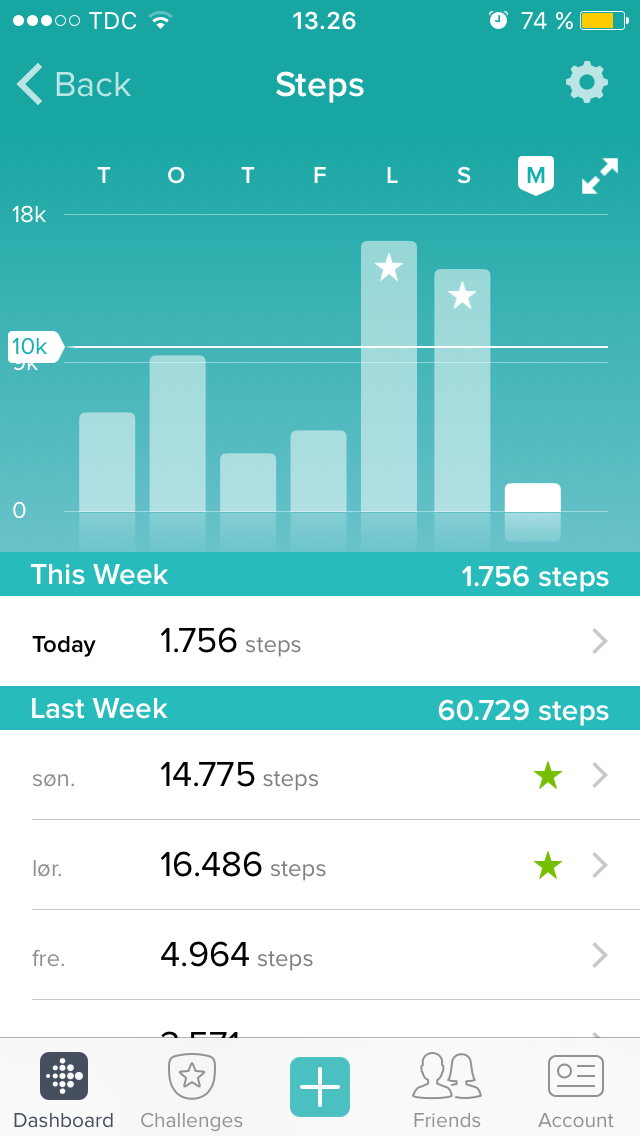
\includegraphics[width=0.6\textwidth]{figures/brugerfladesteps}
	\caption{Til venstre ses den grafiske oversigt over antal skridt taget, og højre figur viser skridt taget i en tabel.}
	\label{fig:brugerfladesteps}
\end{figure}


 

%	\end{itemize}
%	\item Hvor udbredt er teknologien? (Studier med noget statistik hertil.)
Producenten Fitbit 			
			
			Statistik op aktivitetsarmbånd på verdensplan 
%	\item Aktivitetsarmbånd
%	\begin{itemize}
%		\item Hvilke sensor bliver brugt til at opsamle data

%		\item Et billede hertil!
%	\end{itemize}
%	\item Hvordan monteres/påføres teknologien 
%	\item Hvordan kalibreres teknologien til den enkelte person?
%	\begin{itemize}
%		\item Skal der udføres nogle test for at vide f.eks. hvilepulsen hos patienten? i så fald hvordan gøres dette?
%	\end{itemize}
%	\item Levetid for teknologien (Evt. Batterilevetid/Totale levetid)
%	\item Hvordan lagres og videregives informationen til en læge?
\end{itemize}